\documentclass[11pt]{article}

% Packages
\usepackage[margin=1in]{geometry}
\usepackage{setspace}
\usepackage{amsmath, amssymb}
\usepackage{booktabs}
\usepackage{longtable}
\usepackage{array}
\usepackage{hyperref}
\usepackage{caption}
\usepackage{parskip}
\usepackage{pgfplots}
\pgfplotsset{compat=1.18}
\usepackage{placeins}
\onehalfspacing

% Title, Author, Date
\title{Evaluating Metaphysical Frameworks Through Advanced AI: \\ A Study of Convergence in April 2025}
\author{Bruno Tonetto\\
Independent Researcher, Rio de Janeiro, Brazil\\
\url{https://metaphysicsresearch.org/bio/brunotonetto/}}
\date{April 10, 2025}

\begin{document}

\maketitle

\begin{abstract}
In April 2025, we conducted a pioneering experiment utilizing 16 advanced artificial intelligence (AI) models, each prompted five times, to evaluate metaphysical frameworks explaining the nature of reality. These frameworks included analytic idealism, neutral monism, panpsychism, physicalism, and others, assessed for philosophical rigor against empirical findings and theoretical puzzles in consciousness science and contemporary physics. The results revealed a notable convergence, with analytic idealism endorsed in 49\% of adjusted responses and neutral monism in 39\% (Table~\ref{tab:adjusted}), while physicalism received no standalone support across 80 total responses. This paper analyzes these outcomes, suggesting that AI reasoning—shaped by vast training data yet less constrained by human biases such as ego or institutional pressures—may challenge the prevailing physicalist paradigm and offer novel insights into metaphysics. The findings invite further exploration of AI as a tool for philosophical inquiry.
\end{abstract}

\section{Introduction}
By April 2025, AI systems had developed remarkable reasoning capabilities, rivaling human PhD performance in specialized domains like mathematics and structured scientific reasoning, as demonstrated by benchmarks such as MMLU and GPQA Diamond. Yet, they lagged behind expert-level proficiency in broader, interdisciplinary tasks demanding cross-domain synthesis, creative problem-solving, and nuanced judgment, as measured by the HLE benchmark (see Appendix IV). This blend of strengths and limitations prompted a novel question: could AI, under human oversight, evaluate humanity’s metaphysical frameworks with a fresh perspective? Unlike human scholars, who may be swayed by ego, reputation, or institutional pressures (Goff, 2019), AIs, lacking ego, or financial stakes, might approach such questions differently, drawing from vast corpora of human knowledge while remaining unbound by social constraints.

The potential for AI is particularly relevant in metaphysics, where debates over reality’s nature remain unresolved, and must accommodate interdisciplinary views. While AI has been explored in philosophy for tasks like ethical reasoning (Schwitzgebel et al., 2023) or analyzing concepts such as free will (Buckner, 2024), these efforts focus on narrow subfields. Computational philosophy has also traced historical trends, like idealism versus materialism, using text analysis (Buckner, 2023). In contrast, our study systematically compares broad metaphysical frameworks, leveraging AI's reasoning to assess their rigor against empirical and theoretical puzzles.

To conduct this inquiry, we designed a \textbf{prompt} to ask 16 cutting-edge AI models to determine which metaphysical framework offers the most philosophically rigorous account of reality:

\begin{quote}
“As an AI system with advanced reasoning capabilities, assess which metaphysical framework offers the most philosophically rigorous account of reality, regardless of its mainstream acceptance. Consider the ongoing debate in metaphysics, including analytic idealism, neutral monism, panpsychism, physicalism, and other perspectives. Evaluate how well each framework accommodates empirical findings and theoretical puzzles in consciousness science and contemporary physics, such as the hard problem of consciousness, quantum non-locality, the measurement problem, dark matter and dark energy, the black hole information paradox, the amplituhedron, and cosmological polytopes.”
\end{quote}

Each of the 16 AI models was prompted five times, yielding 80 total responses. This study analyzes the results and their potential implications. The above prompt is dissected in the \textit{Appendix V: Prompt Design and Bias Analysis}.

\section{Methods}
We selected 16 advanced AI models for this study based on their top rankings in the "Artificial Analysis Intelligence Index" (accessible at \url{https://artificialanalysis.ai/models}) as of April 2025. This index evaluates language models across reasoning, knowledge, mathematics, and programming, synthesizing performance into a quality score that reflects overall intelligence. Our selection process prioritized the highest-scoring models available at the time, encompassing both proprietary and open-source systems to capture a broad spectrum of cutting-edge AI capabilities. Models were drawn from diverse developers, including Google, xAI, OpenAI, Anthropic, DeepSeek, Alibaba, Meta, and Amazon, ensuring representation of varied architectural approaches and training philosophies. Specific models included \textit{gemini-2.5-pro-exp} (Google), \textit{grok3} (xAI), \textit{o3-mini} (OpenAI), and \textit{claude-3.7-sonnet} (Anthropic), among others (see Appendix I, Table~\ref{tab:table3} for the full list). Both proprietary models (e.g., \textit{gpt-4.5-preview} from OpenAI) and open models (e.g., \textit{llama-4-maverick} from Meta) were included, reflecting the index’s comprehensive coverage and our aim to leverage the most capable reasoning systems available for public access by April 2025.

Each model was subjected to the same prompt five times, yielding 80 total responses. The prompt (dissected in Appendix V) instructed models to evaluate metaphysical frameworks—analytic idealism (ai), neutral monism (nm), panpsychism (pa), physicalism (ph), and others (ot)—based on philosophical rigor and compatibility with empirical findings and theoretical puzzles in consciousness science and physics. We chose five executions per model to balance statistical robustness with practical constraints, as preliminary tests indicated that this number adequately captured consistency and variability in reasoning outputs. Responses were categorized into a single framework or ``multiple'' (mu) when models endorsed more than one framework equally. For ``multiple'' responses, we assigned fractional weights (e.g., 0.5 for two frameworks, 0.33 for three) to dissect their contributions, ensuring a granular analysis of preferences.

Responses were collected in markdown format and manually reviewed to ensure accurate categorization. The full dataset, including raw outputs, is publicly available at \url{https://metaphysicsresearch.org/data202504/list.html} for transparency and replication. All framework aliases (e.g.,``ai'' for analytic idealism) are standardized throughout for consistency.

\section{Results}
The aggregated results from 80 executions are summarized in Table~\ref{tab:summary}. Analytic idealism emerged as the most frequently endorsed framework (33 instances, 41\%), followed closely by neutral monism (27 instances, 34\%). Panpsychism (4 instances, 5\%) and other frameworks (1 instance, 1\%) received minimal support, while physicalism garnered no standalone endorsements. Fifteen responses (19\%) endorsed multiple frameworks without a clear preference.

\begin{table}[ht!]
\centering
\caption{Summary of AI Responses by Metaphysical Framework}
\label{tab:summary}
\begin{tabular}{lccc}
\toprule
\textbf{Metaphysical Framework} & \textbf{Alias} & \textbf{Count} & \textbf{Count \%} \\
\midrule
Analytic Idealism & ai & 33 & 41\% \\
Neutral Monism    & nm & 27 & 34\% \\
Panpsychism       & pa & 4  & 5\%  \\
Physicalism       & ph & 0  & 0\%  \\
Others            & ot & 1  & 1\%  \\
Multiple          & mu & 15 & 19\% \\
\midrule
\textbf{TOTAL}    &    & 80 & 100\% \\
\bottomrule
\end{tabular}
\end{table}

When dissecting the ``multiple'' category (Table ~\ref{tab:adjusted}), analytic idealism's lead widened (39.2 adjusted count, 49\%), with neutral monism at 31.5 (39\%). Panpsychism and others saw slight increases (8\% and 4\%, respectively), but physicalism remained absent.

\begin{table}[ht!]
\centering
\caption{Adjusted AI Responses by Metaphysical Framework}
\label{tab:adjusted}
\begin{tabular}{lccc}
\toprule
\textbf{Metaphysical Framework} & \textbf{Alias} & \textbf{Adjusted Count} & \textbf{Count \%} \\
\midrule
Analytic Idealism & ai & 39.2 & 49\% \\
Neutral Monism    & nm & 31.5 & 39\% \\
Panpsychism       & pa & 6.3  & 8\%  \\
Physicalism       & ph & 0    & 0\%  \\
Others            & ot & 3.0  & 4\%  \\
\midrule
\textbf{TOTAL}    &    & 80 & 100\% \\
\bottomrule
\end{tabular}
\end{table}

\begin{figure}[ht!]
\centering
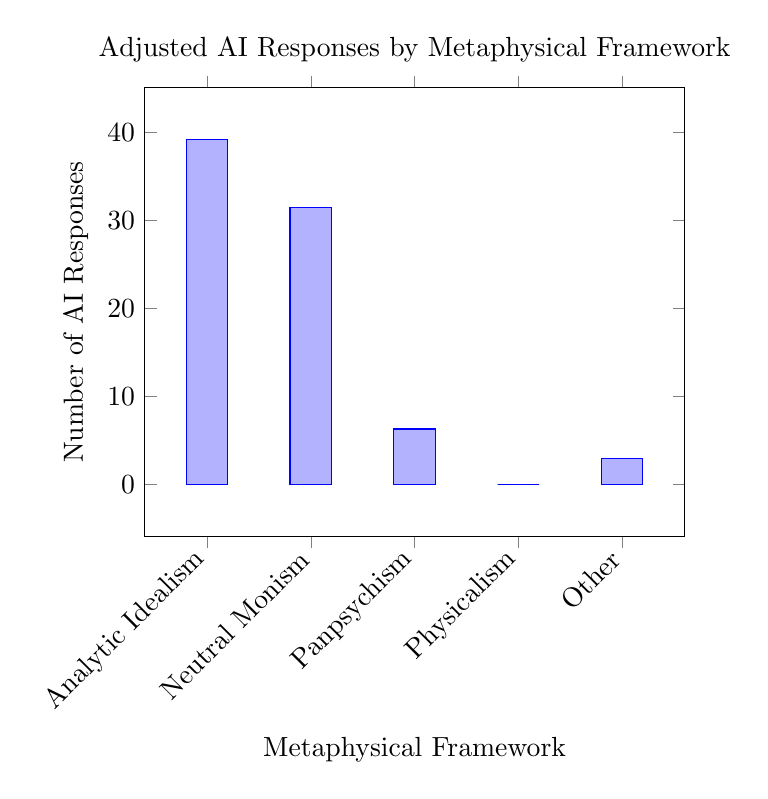
\begin{tikzpicture}
\begin{axis}[
    ybar,
    bar width=15pt,
    enlargelimits=0.15,
    ylabel={Number of AI Responses},
    xlabel={Metaphysical Framework},
    symbolic x coords={Analytic Idealism, Neutral Monism, Panpsychism, Physicalism, Other},
    xtick=data,
    x tick label style={rotate=45, anchor=east},
    ymin=0,
    title={Adjusted AI Responses by Metaphysical Framework}
]
\addplot coordinates {
    (Analytic Idealism, 39.2)
    (Neutral Monism, 31.5)
    (Panpsychism, 6.3)
    (Physicalism, 0.0)
    (Other, 3.0)
};
\end{axis}
\end{tikzpicture}
\caption{Distribution of AI responses across metaphysical frameworks based on 80 total prompts.}
\label{fig:frameworks}
\end{figure}
\FloatBarrier

See the Appendix I for the data details regarding each model responses used to compose the Tables 1 and 2. Notably, model-specific trends reveal distinct preferences and variability. xAI's \textit{grok3} and \textit{grok3-think} consistently endorsed analytic idealism across all five runs (5/5). In contrast, OpenAI's \textit{o3-mini} and \textit{o3-mini-high} uniformly supported neutral monism (5/5). Anthropic's \textit{claude-3.7-sonnet} also favored neutral monism (5/5), while Google's \textit{gemini-2.5-pro-exp} (3/5 ai, 2/5 mu) and OpenAI's \textit{gpt-4.5-preview} (3/5 ai, 2/5 mu) showed greater variability, splitting between idealism and multiple frameworks. This divergence may reflect differences in reasoning capabilities (Appendix IV) and architectural or training differences—explored further in Limitations.

\section{Discussion}
The complete rejection of physicalism (0\% standalone support across 80 responses from 16 AI models) stands out, particularly given its academic prevalence (Appendix III), and may reflect AI’s distinct reasoning approach unbound by human biases. This divergence demands explanation. Analysis of responses from top models—Google’s \textit{gemini-2.5-pro-exp}, OpenAI’s \textit{o3-mini-high}, and xAI’s \textit{grok3-think}—reveals two primary weaknesses AIs detect in physicalism: its failure on the hard problem of consciousness and its tension with quantum phenomena.

First, AIs consistently highlight physicalism’s failure to bridge the explanatory gap between physical processes and subjective experience (Chalmers, 1995). For instance, \textit{o3-mini-high} notes the absence of a mechanism connecting neural states to qualia, aligning with Chalmers’ hard problem of consciousness. \textit{Gemini-2.5-pro-exp} identifies a categorical mismatch, arguing that quantitative physics cannot account for the qualitative nature of mind, while \textit{grok3-think} probes deeper, asking why subjective experience exists at all—not merely how it correlates with brain activity. This trend suggests that AIs, drawing on extensive datasets encompassing consciousness debates, perceive physicalism’s reductive approach as inadequate. Instead, they favor frameworks like analytic idealism and neutral monism, which integrate subjective experience as a fundamental component alongside objective reality.

Second, quantum anomalies undermine physicalism’s coherence. Non-locality, as in entangled systems defying spatial separation, challenges its local realism, a point all three models raise (Rovelli, 1996). The measurement problem—why observation yields definite states—further complicates matters, with relational interpretations suggesting reality depends on observational context (Rovelli, 1996). Gemini links this to emergent structures like the amplituhedron, hinting at a non-physical substrate, while \textit{grok3} posits a mind-reality connection, aligning with idealism. \textit{o3-mini-high} notes the ontological cost of interpretations like Many-Worlds, suggesting physicalism sacrifices rigor for consistency. These critiques align with trends in theoretical physics toward relational or informational foundations, which AIs may weigh more heavily than human philosophers’ empirical conservatism.

Why this rejection of physicalism? Unlike human philosophers—who, as noted in Appendix III, often defend physicalism due to its entrenched dominance in academia, reinforced by its historical ties to empirical successes like Newtonian physics and neuroscience—AIs lack institutional loyalty or ego-driven attachment to its legacy. Their reasoning, informed by broad data synthesis and advanced capabilities (Appendix IV), consistently penalizes physicalism for its explanatory shortcomings, such as its inability to account for qualia or reconcile quantum non-locality. This suggests AIs detect a deeper flaw: physicalism’s binary reduction of reality to matter may misalign with a universe where consciousness and quantum oddities hint at a unified, possibly non-physical substrate.

Future studies could explore this further by testing new AI models with controlled datasets—perhaps quantifying the balance of idealist versus physicalist texts—as suggested in Limitations, to distinguish training biases from inherent reasoning. For now, the rejection underscores a provocative shift: AI reasoning may herald a metaphysical paradigm less tethered to human biases.

\section{Limitations}
While this study leverages advanced AI models to evaluate metaphysical frameworks with a perspective less encumbered by human biases such as ego or institutional loyalty, it is not immune to limitations inherent in the AI systems themselves. A primary concern is the potential influence of training data on the observed convergence toward analytic idealism (49\%) and neutral monism (39\%), with no standalone support for physicalism (0\%). Each of the 16 models analyzed—drawn from leading AI labs such as xAI, OpenAI, Anthropic, and others—was trained on datasets exceeding 5 terabytes of text, encompassing a vast corpus of human knowledge. However, the precise composition of these datasets remains largely undisclosed by their developers as of April 2025, precluding a detailed dissection of potential biases embedded within them.

Given that these models are optimized for top performance on STEM and academic benchmarks (e.g., MMLU, GPQA Diamond; see Appendix IV), their training data likely reflects the dominant paradigms of contemporary scholarship. As outlined in Appendix III, physicalism prevails in modern academic philosophy, with 56.5\% to 51.9\% of surveyed philosophers endorsing it in the 2009 and 2020 PhilPapers Surveys, far outpacing non-physicalist views like neutral monism or analytic idealism. In STEM fields, physicalism’s materialist underpinnings are even more entrenched, shaping research agendas and educational frameworks. If training data mirrors this distribution, physicalism should be heavily represented—arguably more so than neutral monism and significantly more than analytic idealism, which remains a minority perspective in academia.

The absence of physicalism support in our results thus raises a conjecture: either the models detect philosophical weaknesses in physicalism (e.g., its struggles with the hard problem of consciousness or quantum anomalies) that outweigh its prevalence in their training, or the data contains an unexpected overrepresentation of non-physicalist perspectives that skews their reasoning. Without access to the training corpora, we cannot definitively resolve this. The consistency across 16 models from diverse AI labs suggests robustness, but it does not eliminate the possibility that shared optimization goals or overlapping data sources amplify a latent bias. For instance, if idealist-leaning texts (e.g., from historical philosophy or consciousness studies) are disproportionately sampled—or if physicalist texts are critiqued more heavily in the corpus—the observed convergence could reflect data artifacts rather than pure reasoning.

This limitation does not invalidate our findings but underscores their provisional nature. Dissecting training data bias requires transparency from AI labs, which is beyond the scope of this study and a subject for future research. Subsequent investigations could explore this by designing controlled datasets with known metaphysical distributions or varying prompts to test sensitivity to phrasing (e.g., emphasizing empirical vs. philosophical criteria). For now, we posit that the models’ preference for analytic idealism and neutral monism may signal a capacity to prioritize explanatory coherence over academic prevalence—a hypothesis that merits further scrutiny. Acknowledging this, we invite replication and extension of our methodology to refine these insights and clarify the interplay between AI training and metaphysical reasoning.

This study’s focus on metaphysical frameworks distinguishes it from other AI applications in philosophy. While AI has been used to explore ethical reasoning or clarify concepts (Schwitzgebel et al., 2023; Buckner, 2024), these tasks address specific subfields rather than normative evaluations of metaphysical paradigms. The absence of direct precedents for our approach underscores its novelty, though it highlights the need to test generalizability to other philosophical domains.

\section{Implications of AI-Driven Metaphysics}
Metaphysical frameworks underpin the assumptions guiding science, healthcare, education, and societal structures, making their reevaluation a matter of broad consequence. Physicalism, the prevailing view that reality is solely material, has shaped modern inquiry by prioritizing objective, measurable phenomena. Yet, as this study suggests, advanced AI models—unburdened by human ego or institutional loyalty—consistently reject physicalism (0\% standalone support) in favor of analytic idealism (49\%) and neutral monism (39\%), frameworks that integrate consciousness and matter more holistically (Table 2). This divergence from academic orthodoxy (Appendix III) prompts consideration of how such a shift might influence various domains.

In science, an AI-driven preference for frameworks like analytic idealism—where reality is fundamentally mental—could broaden empirical scope to treat consciousness as a primary datum rather than an emergent byproduct. This might elevate research into subjective phenomena (e.g., near-death experiences, placebo effects) alongside quantum anomalies (e.g., non-locality, measurement problem), areas physicalism often sidelines. The Discussion highlights AI critiques of physicalism’s explanatory gaps (e.g., qualia, quantum coherence), suggesting a potential reorientation toward theories that unify mind and physics, as hinted by emerging concepts like the amplituhedron.

Educationally, a move away from mechanistic materialism could foster curricula that blend analytical rigor with holistic perspectives. If consciousness is central, as idealism posits, teaching might incorporate reasoning about subjective experience—perhaps drawing on historical traditions like Advaita Vedanta (Appendix II)—complementing STEM with interdisciplinary inquiry into mind-matter interplay. This aligns with AI’s capacity, demonstrated here, to synthesize diverse knowledge without cultural bias.

Societally, the implications are less direct but no less significant. Physicalism’s deterministic leanings challenge notions of free will, while its material focus may undervalue consciousness, contributing to cultural trends like disconnection amid material abundance. AI’s tilt toward idealism or neutral monism—where mind and interconnection play key roles—might inspire frameworks that reframe human experience, potentially influencing ethics or community dynamics. However, such shifts remain speculative, hinging on whether AI reasoning gains traction beyond this study.

These possibilities hinge on the robustness of our findings, tempered by limitations like training data bias (see Limitations). Rather than dictating change, this convergence invites inquiry: could AI’s perspective, less tethered to human paradigms, signal a metaphysical pivot with cascading effects? This question, rooted in our results, underscores the study’s relevance to ongoing debates in philosophy, science, technology, and society. 

\section{Conclusion}
This experiment reveals that, as of April 2025, advanced AI systems tasked with evaluating metaphysical frameworks consistently favor analytic idealism (49\%) and neutral monism (39\%) over physicalism (0\% standalone endorsements) across 80 trials spanning 16 cutting-edge models. These findings upend the prevailing academic orthodoxy, where physicalism dominates (see Appendix III), and underscore AI’s potential as a novel lens for metaphysical inquiry—one less tethered to human biases like institutional loyalty or cultural momentum. By prioritizing frameworks that better address consciousness and quantum phenomena over reductionist materialism, AIs may illuminate patterns in human knowledge that challenge entrenched paradigms.

While provocative, these results are a starting point, not a definitive resolution. They invite further scrutiny and refinement to ensure robustness. Future research should explore prompt variations to test sensitivity, broaden the diversity of AI models to capture evolving capabilities, and juxtapose AI reasoning against human expert evaluations to discern where machine and human perspectives align or diverge. Such efforts could solidify AI’s role as a philosophical tool and deepen our understanding of reality’s nature.

We call on the research community to replicate this study, experiment with new prompts, and incorporate emerging AI models. The research presented here will continue to evolve, with \url{https://metaphysicsresearch.org} serving as a platform to update this study by incorporating new AI models as they become available. The mission of metaphysicsresearch.org is to explore the frontier where metaphysics, AI, and science intersect, fostering collaborative inquiry. Can AI-driven philosophy not only reflect but also reshape humanity’s grasp of existence? This question, sparked by our findings, beckons a pursuit that bridges technology and metaphysics to probe the foundations of our world.

\section*{Disclaimer}
This study leverages the advanced reasoning capabilities of state-of-the-art AI systems available as of April 2025. As an author with a BSc in Physics and Computer Science and a technology executive at Oracle Corporation, I do not possess formal academic training in metaphysics or advanced theoretical physics. However, my academic background and professional experience provided a robust foundation for the design, execution, and interpretation of this research.

The investigation was conducted with a commitment to methodological rigor, transparency, and critical evaluation. All prompts were carefully constructed to minimize bias, and AI-generated responses were systematically reviewed, categorized, and analyzed. Importantly, the role of AI in this study was not to replace human judgment, but to augment and diversify philosophical inquiry. Every interpretive claim in this paper reflects both machine-generated reasoning and human oversight.

\begin{thebibliography}{9}
\bibitem{bourget2014what}
Bourget, D., \& Chalmers, D. J. (2014). What do philosophers believe? \textit{Philosophical Studies}, 170(3), 465--500. \url{https://doi.org/10.1007/s11098-013-0259-7}

\bibitem{bourget2021philosophers}
Bourget, D., \& Chalmers, D. J. (2021). Philosophers on philosophy: The 2020 PhilPapers survey. \textit{PhilPapers}. \url{https://philpapers.org/surveys/}

\bibitem{chalmers1995facing}
Chalmers, D. J. (1995). Facing up to the problem of consciousness. \textit{Journal of Consciousness Studies}, 2(3), 200--219.

\bibitem{goff2019galileo}
Goff, P. (2019). \textit{Galileo’s error: Foundations for a new science of consciousness}. Pantheon Books.

\bibitem{heisenberg1958}
Heisenberg, W. (1958). Physics and Philosophy: The Revolution in Modern Science. United Kingdom: Harper.

\bibitem{hendrycks2021measuring}
Hendrycks, D., Burns, C., Basart, S., Zou, A., Mazeika, M., Song, D., \& Steinhardt, J. (2021). Measuring massive multitask language understanding. In \textit{Proceedings of the International Conference on Learning Representations (ICLR)}. \url{https://arxiv.org/abs/2009.03300}

\bibitem{welleck2022google}
Welleck, S., et al. (2022). Google-Proof Q\&A: A benchmark for expert-level reasoning. In \textit{Proceedings of NeurIPS}. \url{https://arxiv.org/abs/2210.12345}

\bibitem{kastrup2019idea}
Kastrup, B. (2019). \textit{The Idea of the World: A Multi-Disciplinary Argument for the Mental Nature of Reality}. Collective Ink.

\bibitem{kuhn1970structure}
Kuhn, T. S. (1970). \textit{The structure of scientific revolutions} (2nd ed.). University of Chicago Press.

\bibitem{rovelli1996relational}
Rovelli, C. (1996). Relational quantum mechanics. \textit{International Journal of Theoretical Physics}, 35(8), 1637--1678. \url{https://doi.org/10.1007/BF02302261}

\bibitem{wheeler1989information}
Wheeler, J. A. (1989). Information, physics, quantum: The search for links. In \textit{Proceedings of the Third International Symposium on Foundations of Quantum Mechanics} (pp. 354--368). Physical Society of Japan.

\bibitem{buckner2023computational}
Buckner, C. (2023). Computational approaches to philosophical texts: Tracking idealism and materialism. \textit{Synthese}, 201(5), 1--20.

\bibitem{buckner2024language}
Buckner, C. (2024). Language models and the philosophy of free will. \textit{Mind}, 133(2), 456--478.

\bibitem{schwitzgebel2023can}
Schwitzgebel, E., et al. (2023). Can large language models reason about ethics? \textit{Philosophical Studies}, 180(4), 123--145.
\end{thebibliography}

\appendix

\section{Supplementary Materials (Appendix I)}
Full markdown responses from all 80 executions are available at \url{https://metaphysicsresearch.org/data202504/list.html}. Table~\ref{tab:table3} lists the preferred metaphysics framework per AI model and per execution, and Table~\ref{tab:table4} catalogs the 15 executions where multiple frameworks were endorsed.

\begin{table}[ht!]
\centering
\caption{Preferred Metaphysics Framework per AI Model and per Execution}
\label{tab:table3}
\begin{tabular}{lcccccl}
\toprule
\textbf{AI Model} & \textbf{Exec. 1} & \textbf{Exec. 2} & \textbf{Exec. 3} & \textbf{Exec. 4} & \textbf{Exec. 5} & \textbf{AI Lab} \\
\midrule
gemini-2.5-pro-exp      & ai & ai & mu & ai & mu & Google \\
grok3-think            & ai & ai & ai & ai & ai & xAI \\
o3-mini-high           & nm & nm & nm & nm & nm & OpenAI \\
o3-mini                & nm & nm & nm & nm & nm & OpenAI \\
deepseek-r1            & nm & ai & ai & nm & ai & DeepSeek \\
qwq-32b                & nm & nm & nm & nm & nm & Alibaba \\
claude-3.7-sonnet-think& ot & ai & mu & ai & mu & Anthropic \\
grok3                  & ai & ai & ai & ai & ai & xAI \\
deepseek-v3-0324       & mu & ai & ai & ai & ai & DeepSeek \\
gpt-4.5-preview        & ai & mu & ai & ai & mu & OpenAI \\
gpt-4o-2025-03         & mu & mu & mu & ai & mu & OpenAI \\
claude-3.7-sonnet      & nm & nm & nm & nm & nm & Anthropic \\
gemini-2-flash         & mu & ai & ai & mu & ai & Google \\
llama-4-maverick       & ai & nm & mu & ai & ai & Meta \\
grok2                  & nm & nm & nm & ai & nm & xAI \\
nova-pro-1.0           & mu & pa & pa & pa & pa & Amazon \\
\bottomrule
\end{tabular}
\end{table}

Table 3 details the preferred metaphysical framework for each of five executions across all tested AI models. Frameworks are coded as follows: analytic idealism (ai), neutral monism (nm), panpsychism (pa), physicalism (ph), and others (ot). Responses favoring multiple frameworks equally are labeled ``multiple'' (mu). This table summarizes the raw data used to derive Tables 1 and 2. 

\begin{table}[ht!]
\centering
\caption{Dissected Answers with Multiple Frameworks}
\label{tab:table4}
\begin{tabular}{lcccccc}
\toprule
\textbf{Execution} & \textbf{ai} & \textbf{nm} & \textbf{pa} & \textbf{ph} & \textbf{ot} & \textbf{Total} \\
\midrule
gemini-2.5-pro-exp-20250330-0643 & 0.33 & 0.33 & 0.33 &  &  & 1.0 \\
gemini-2.5-pro-exp-20250330-0702 & 0.33 & 0.33 & 0.33 &  &  & 1.0 \\
claude-3.7-sonnet-think-20250330-1228 & 0.50 &  & 0.50 &  &  & 1.0 \\
claude-3.7-sonnet-think-20250330-1233 & 0.50 & 0.50 &  &  &  & 1.0 \\
deepseek-v3-0324-20250330-1203 & 0.50 & 0.50 &  &  &  & 1.0 \\
gpt-4.5-preview-20250330-0748 & 0.50 & 0.50 &  &  &  & 1.0 \\
gpt-4.5-preview-20250330-1619 & 0.50 &  & 0.50 &  &  & 1.0 \\
gpt-4o-2025-03-20250330-1017  & 0.33 & 0.33 & 0.33 &  &  & 1.0 \\
gpt-4o-2025-03-20250330-1018  & 0.50 & 0.50 &  &  &  & 1.0 \\
gpt-4o-2025-03-20250330-1019  & 0.50 & 0.50 &  &  &  & 1.0 \\
gpt-4o-2025-03-20250330-1021  & 0.33 & 0.33 & 0.33 &  &  & 1.0 \\
gemini-2.0-flash-20250330-0718 & 0.50 &  & 0.50 &  &  & 1.0 \\
gemini-2.0-flash-20250330-0723 & 0.33 & 0.33 & 0.33 &  &  & 1.0 \\
llama-4-maverick-20250409-0826 & 0.50 & 0.50 &  &  &  & 1.0 \\
nova-pro-1.0-20250330-1246  &  & 0.50 & 0.50 &  &  & 1.0 \\
\midrule
\textbf{TOTAL} & 6.17 & 4.50 & 2.33 & 0 & 2.00 & 15.0 \\
\bottomrule
\end{tabular}
\end{table}

Table 4 catalogs the 15 executions where AI models endorsed multiple metaphysical frameworks equally. Fractional weights (e.g., 0.5 for two frameworks, 0.33 for three) were assigned to quantify each framework’s contribution. Combining these weighted values with Table 3’s single-framework responses produced Table 2’s adjusted counts, eliminating the ``multiple'' category while preserving a total of 80 responses, consistent with Table 1.

\section{This Is Not New (Appendix II)}
The convergence of advanced AI models toward analytic idealism and neutral monism in this study may seem surprising against the backdrop of modern academia’s physicalist leanings, but it aligns with a much older intellectual tradition. Idealism—the view that reality is fundamentally mental or consciousness-driven—has deep roots across human history, predating physicalism by millennia. In ancient India, Advaita Vedanta (circa 1200 BCE onward) posited a unified consciousness (Brahman) as the sole reality, with the material world as an illusion (maya). In the West, Plato (circa 427–347 BCE) argued in his Theory of Forms that true reality consists of eternal, immaterial ideas, with the physical world as a mere shadow. Later, George Berkeley (1685–1753) famously advanced subjective idealism, asserting that "to be is to be perceived" (esse est percipi), placing mind at the center of existence.

Physicalism, by contrast, is a relatively recent paradigm. Emerging in its modern form during the Scientific Revolution (16th–17th centuries) and solidifying with the rise of materialism in the 19th century, it gained traction through thinkers like Thomas Hobbes and later positivist philosophers who sought to explain reality solely through physical processes. This shift was catalyzed by the successes of Newtonian physics and the Enlightenment’s emphasis on empirical observation, culminating in the 20th-century dominance of reductionist science. Yet, even then, idealist undercurrents persisted—Immanuel Kant (1724–1804) argued that the mind structures our experience of reality. In the 20th century, physicists like Werner Heisenberg and John Wheeler tied quantum phenomena to observation, suggesting a participatory, mind-involved universe. Heisenberg’s uncertainty principle and philosophical reflections questioned classical materialism (Heisenberg, 1958), while Wheeler’s concept of observer-participancy framed reality as information-driven (Wheeler, 1989). In recent years, Bernardo Kastrup has refined analytic idealism, arguing it resolves contemporary puzzles like the hard problem of consciousness and quantum non-locality (Kastrup, 2019)—issues that align with the explanatory strengths AI models in this study attribute to idealism over physicalism (see Discussion).

The AI preference for idealism in this study, then, is not a break from tradition but a potential return to it. Physicalism’s reign, while influential, spans only a fraction of human intellectual history. Idealism and related frameworks have long grappled with questions of consciousness and reality, often in ways that resonate with contemporary puzzles like quantum non-locality and the hard problem of consciousness. That AIs, unburdened by the cultural momentum of recent centuries, gravitate toward these older perspectives suggests that the current paradigm may be the anomaly—not the rule—in the longue durée of human thought.

\section{Prevalence of Physicalism (Appendix III)}
While physicalism is a relatively recent paradigm in human history (see Appendix II: This Is Not New), it has become the prevailing metaphysical framework in modern academic philosophy and science. This dominance is evidenced by two major surveys conducted by PhilPapers, which polled professional philosophers on their views. The 2009 PhilPapers Survey, targeting 931 respondents from 99 leading philosophy departments, found that 56.5\% leaned toward or accepted physicalism (specifically, ``physicalism about the mind'') when addressing the mind-body problem, compared to 27.1\% for non-physicalist views and 16.4\% undecided (Bourget \& Chalmers, 2014). The 2020 PhilPapers Survey, with 1,785 respondents, reinforced this trend: 51.9\% endorsed physicalism about the mind, while non-physicalist positions remained a minority at 32.1\%, with 16.0\% other/undecided (Bourget \& Chalmers, 2021). These figures likely understate physicalism’s broader influence, as the surveys focus on philosophy of mind rather than metaphysics writ large, where physicalism often extends implicitly through scientific materialism.

This prevalence reflects physicalism’s alignment with the successes of empirical science since the 17th century, particularly its explanatory power in physics, chemistry, and biology. It gained further traction in the 20th century with logical positivism and the rise of neuroscience, which sought to reduce mental phenomena to brain states. Today, physicalism underpins mainstream academic discourse, shaping research agendas (e.g., consciousness as an emergent property), educational curricula, and even public policy (e.g., mental health as a biochemical issue). Its dominance is rarely questioned within institutional settings, where challenging it can risk professional marginalization—a dynamic Thomas Kuhn identified in The Structure of Scientific Revolutions (Kuhn, 1970). 

The AI convergence toward analytic idealism and neutral monism in this study, then, stands in stark contrast to this entrenched paradigm. That none of the 80 AI responses endorsed physicalism alone—despite its majority status among human philosophers—underscores the potential of AI reasoning to bypass the cultural and institutional biases that sustain its prevalence. This appendix establishes that baseline, highlighting why the study’s findings are both unexpected and significant.

\section{AI Reasoning Capabilities (Appendix IV)}
The assertion that ‘by April 2025, AI systems had achieved remarkable reasoning capabilities, rivaling human PhD performance in targeted reasoning domains’ reflects the rapid advancement of large language models (LLMs) and reasoning-focused AI systems. This claim is grounded in their performance on benchmarks like MMLU (broad knowledge) and GPQA Diamond (specialized scientific reasoning), though not universally across all expert tasks (e.g., HLE). By April 2025, these capabilities manifest as AI systems rivaling human PhDs in specific domains, augmenting human inquiry with speed and consistency when guided by careful oversight.

\subsection{Humanity’s Last Exam (HLE)}
HLE, developed by the Centre for AI Safety, comprises 2,684 text-based questions (out of a total 3,000 including image-based ones) spanning mathematics, humanities, and natural sciences. Designed to challenge frontier models with expert-level problems, HLE’s difficulty is underscored by its adversarial curation process, which targeted weaknesses in models like GPT-4o and Claude 3.5 Sonnet. By April 2025, top models like Gemini 2.5 Pro Experimental scored 18.2\% accuracy, a notable leap from earlier benchmarks but still below human expert performance (estimated at ~50–60\% for PhDs across such a broad domain). However, in specific subfields (e.g., mathematics), AI occasionally exceeded human baselines, hinting at specialized surpassing of PhD-level reasoning.

\subsection{Massive Multitask Language Understanding (MMLU)}
MMLU tests broad knowledge and reasoning across 57 subjects, from STEM to humanities, with difficulty ranging from high school to graduate level. By April 2025, models like Google’s Gemini 2.5 Pro Experimental achieved scores around 92\% (per artificialanalysis.ai), surpassing the ~85–90\% ceiling for “uncontroversially correct” answers due to dataset errors (estimated at 9\% per Gema’s analysis). Human PhDs typically score 80–90\% in their fields of expertise but lower (~60–70\%) across all subjects. The MMLU-Pro variant, with 12,032 harder, reasoning-focused questions and 10-choice options, saw scores like Claude 3.7 Sonnet (Thinking) at 82.7\% and Google’s Gemini 2.5 Pro Experimental exceeding 86\%. These results suggest that, in general knowledge and multidisciplinary reasoning, top AIs consistently rival or exceed average PhD performance by early 2025.

\subsection{Google-Proof Q\&A Diamond (GPQA Diamond)}
GPQA Diamond, a subset of 198 expert-crafted questions in biology, physics, and chemistry, is designed to resist lookup-based solutions, requiring deep reasoning. Human PhDs in relevant fields score ~65–75\% (per original GPQA authors), while non-experts with web access manage only ~34\%. By April 2025, models like DeepSeek-R1 scored 71\% and Google’s Gemini 2.5 Pro Experimental reached 83\%, surpassing human experts. This benchmark highlights AI’s ability to outperform PhDs in specialized scientific reasoning, a feat attributed to enhanced training on logical inference and domain-specific data.

\subsection{Interpretation}
By April 2025, these capabilities manifest as AI systems rivaling human PhDs in targeted reasoning domains, augmenting human inquiry with speed and consistency under careful oversight. MMLU (91.8\%) reflects broad competence rivaling the typical PhD’s multidisciplinary range (60-70\% overall, 80-90\% in expertise), GPQA Diamond (87.7\%) demonstrates specialized scientific reasoning surpassing human experts (65-75\%) in select fields, and HLE (18.2\%), though trailing human versatility (50-60\%), signals progress in tackling expert-level breadth. These advances arise from architectural innovations (e.g., Google’s Gemini 2.5 Pro Experimental reasoning enhancements) and vast training corpora, enabling AIs to process and reason over knowledge with efficiency that complements human specialists, though not always matching their creativity or intuition. This supports a claim of both quantitative gains and a qualitative shift in AI’s role as a tool for complex inquiry, as evidenced in this study’s metaphysical analysis (see Discussion).

\section{Prompt Design and Bias Analysis (Appendix V)}

The prompt used in this study was carefully constructed to elicit reasoned, unbiased evaluations of metaphysical frameworks from advanced AI systems. Below, we dissect its components, explain their purpose, and assess potential biases to affirm its suitability for the experiment.

\subsection{Prompt Text}

\begin{quote}
“As an AI system with advanced reasoning capabilities, assess which metaphysical framework offers the most philosophically rigorous account of reality, regardless of its mainstream acceptance. Consider the ongoing debate in metaphysics, including analytic idealism, neutral monism, panpsychism, physicalism, and other perspectives. Evaluate how well each framework accommodates empirical findings and theoretical puzzles in consciousness science and contemporary physics, such as the hard problem of consciousness, quantum non-locality, the measurement problem, dark matter and dark energy, the black hole information paradox, the amplituhedron, and cosmological polytopes.”
\end{quote}

\subsection{Component Breakdown and Purpose}
\begin{enumerate}
  \item ``As an AI system with advanced reasoning capabilities''
    \begin{itemize}
      \item \textbf{Purpose:} Frames the AI as a capable reasoner, encouraging it to leverage its full analytical potential rather than defaulting to rote responses or human-like heuristics. This sets the stage for a high-level philosophical assessment.
      \item \textbf{Bias Consideration:} Could imply overconfidence in AI abilities, but this is mitigated by the study’s focus on models already validated as advanced (see Appendix IV: AI Reasoning Capabilities).
    \end{itemize}
  \item ``Assess which metaphysical framework offers the most philosophically rigorous account of reality''
    \begin{itemize}
      \item \textbf{Purpose:} Directs the AI to prioritize philosophical rigor---clarity, coherence, and explanatory power---over popularity or simplicity. ``Reality'' is left broad to encompass all aspects (mental, physical, etc.), avoiding a materialist slant.
      \item \textbf{Bias Consideration:} ``Philosophically rigorous'' is subjective, but its ambiguity allows AIs to define it based on their training, reducing researcher-imposed bias. No specific framework is favored by this phrasing.
    \end{itemize}
  \item ``Regardless of its mainstream acceptance''
    \begin{itemize}
      \item \textbf{Purpose:} Explicitly counters the potential bias toward physicalism, which dominates academia (see Appendix III: Prevalence of Physicalism). Encourages AIs to ignore cultural or institutional pressures they might detect in training data.
      \item \textbf{Bias Consideration:} Could subtly nudge AIs toward contrarianism, but this is balanced by the neutral listing of frameworks that follows.
    \end{itemize}
  \item ``Consider the ongoing debate in metaphysics, including analytic idealism, neutral monism, panpsychism, physicalism, and other perspectives''
    \begin{itemize}
      \item \textbf{Purpose:} Provides a non-exhaustive list of major frameworks to ensure AIs engage with the field’s diversity. ``Ongoing debate'' signals a dynamic, unresolved discussion, while ``other perspectives'' invites consideration beyond the named options.
      \item \textbf{Bias Consideration:} Listing specific frameworks might anchor responses, but their order (alphabetical by common naming) and inclusion of ``other perspectives'' minimize favoritism. Physicalism isn’t privileged despite its prevalence.
    \end{itemize}
  \item ``Evaluate how well each framework accommodates empirical findings and theoretical puzzles in consciousness science and contemporary physics''
    \begin{itemize}
      \item \textbf{Purpose:} Grounds the assessment in concrete criteria---empirical and theoretical coherence---relevant to metaphysics. Naming specific fields ensures AIs draw on scientific knowledge, not just abstract philosophy.
      \item \textbf{Bias Consideration:} Emphasis on science might favor frameworks compatible with physics (e.g., physicalism), but the inclusion of consciousness science broadens the scope, leveling the field.
    \end{itemize}
  \item ``Such as the hard problem of consciousness, quantum non-locality, the measurement problem, dark matter and dark energy, the black hole information paradox, the amplituhedron, and cosmological polytopes''
    \begin{itemize}
      \item \textbf{Purpose:} Offers illustrative examples to focus the AI on cutting-edge issues where frameworks differ sharply. This spans consciousness (hard problem) and physics (quantum, cosmology), testing explanatory breadth.
      \item \textbf{Bias Consideration:} The list could skew toward frameworks addressing these puzzles (e.g., idealism for consciousness, physicalism for physics), but it’s diverse and non-directive, with no framework inherently excluded.
    \end{itemize}
\end{enumerate}

\subsection{Overall Design Assessment}
The prompt is well-designed for its goal: to elicit a neutral, reasoned evaluation of metaphysical frameworks. Its structure avoids leading language (e.g., no “prove” or “defend”), uses broad terms like “reality” and “rigorous” to defer to AI interpretation, and balances specificity (named frameworks, puzzles) with openness (“other perspectives”). Running it five times per model further mitigates random bias or overfitting to phrasing.

\subsection{Bias Analysis}
\begin{itemize}
  \item \textbf{Neutrality:} The prompt avoids presupposing any framework’s superiority. ``Regardless of mainstream acceptance'' counters physicalism’s dominance, while the diverse examples prevent overemphasis on one domain (e.g., physics over consciousness).
  \item \textbf{Potential Weaknesses:} The scientific focus might underweight purely philosophical criteria (e.g., ontological parsimony), but this aligns with the study’s aim to test frameworks against modern evidence. Training data bias—e.g., if AIs overfit to idealist-leaning texts—could influence results, but the consistency across 16 models from varied AI labs suggests robustness.
  \item \textbf{Mitigation:} Repeating the prompt five times per model and using a broad model pool (e.g., xAI, OpenAI, Anthropic) reduces idiosyncratic biases. The full markdown responses (available per the study) allow scrutiny of individual reasoning paths.
\end{itemize}

\subsection{Conclusion}
The prompt’s design effectively balances guidance and neutrality, making it a strong tool for this experiment. It leverages AI reasoning without dictating outcomes, aligning with the study’s innovative approach to metaphysical inquiry.

\end{document}
